\section{Transformer Architecture}

\subsection{Overview}

In this section, we break down the components of the transformer model. We cover the overall architecture and key components such as self-attention, multi-head attention, positional encodings, and the feed-forward networks.

The transformer model is built on the idea of self-attention, which allows every position in the input sequence to interact with every other position. This design eliminates the need for sequential processing and enables parallel computation. The model is divided into two main parts, the encoder and the decoder, each consisting of multiple identical layers.

\begin{figure}[htbp]\centering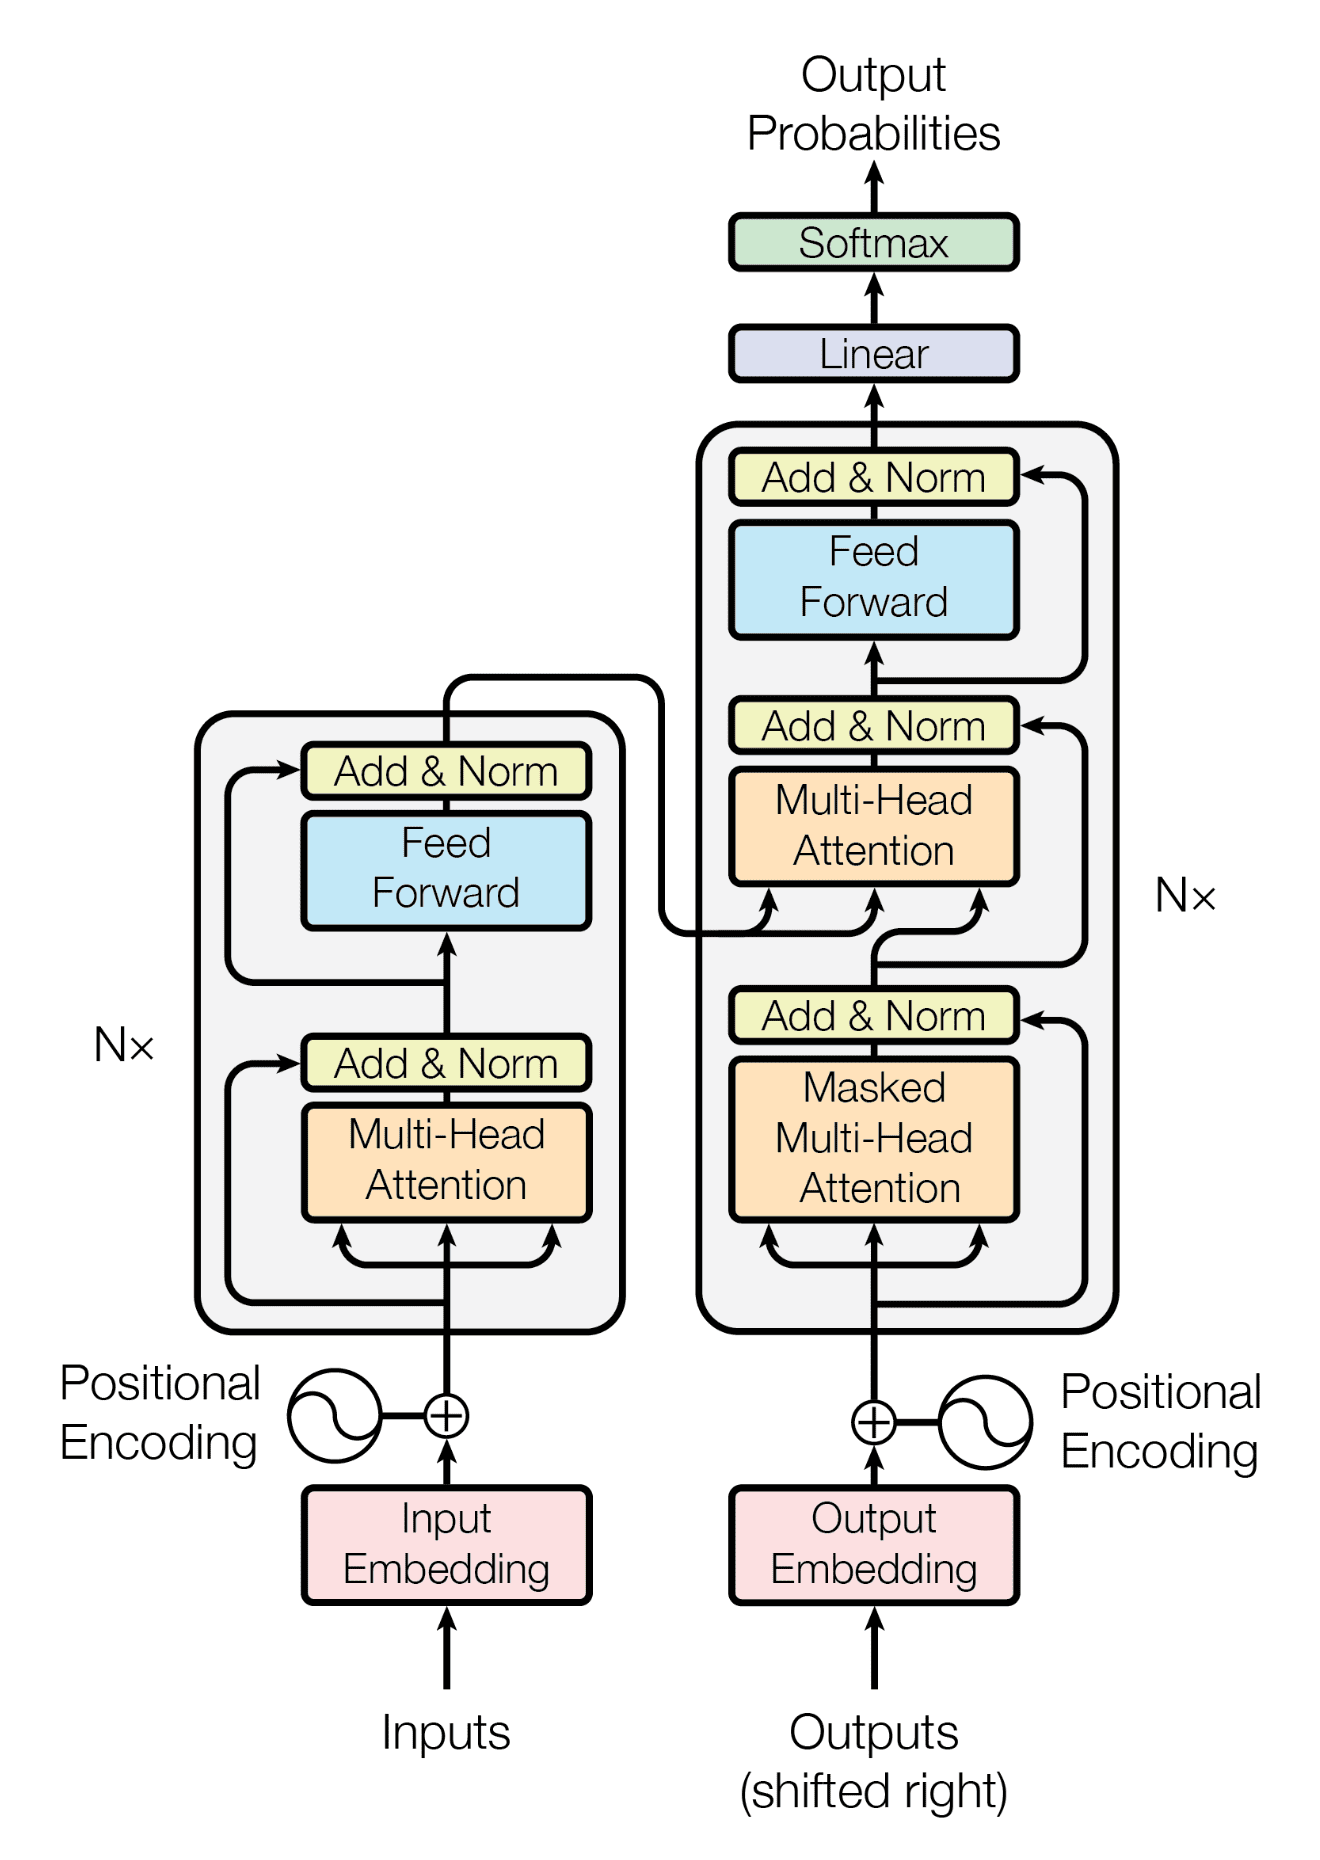
\includegraphics[scale=0.2]{../sections/transformer-architecture/attachments/transformer.png}\caption{The transformer model architecture. The model consists of an encoder (left) and a decoder (right), each containing multiple stacked layers (denoted as N$\times$). The encoder processes input tokens by passing them through embedding layers, positional encoding, multi-head self-attention, and feed-forward networks, with layer normalisation applied after each step. The decoder follows a similar structure but includes an additional masked multi-head attention mechanism to ensure autoregressive generation, preventing positions from attending to future tokens. The final output probabilities are computed through a linear layer and softmax activation.}\label{fig:transformer}\end{figure}

\subsection{Encoder-Decoder Structure}

The encoder transforms an input sequence $\mathbf{X}=(x_1,x_2,\ldots,x_n)$ into a set of continuous representations $\mathbf{H}=(h_1,h_2,\ldots,h_n)$. The decoder then uses $\mathbf{H}$ to generate an output sequence $\mathbf{Y}=(y_1,y_2,\ldots,y_m)$. Each encoder layer is comprised of the following:\begin{enumerate}\item A multi-head self-attention mechanism.\item A position-wise fully connected feed-forward network.\end{enumerate} In the decoder, each layer includes an additional multi-head attention sub-layer that attends over the encoder's output.

\subsection{Self-Attention Mechanism}

The self-attention mechanism allows the model to dynamically focus on different parts of the input sequence. The core operation is the scaled dot-product attention. For given query $\mathbf{Q}$, key $\mathbf{K}$, and value $\mathbf{V}$ matrices, the attention output is computed as \begin{equation}\text{Attention}(\mathbf{Q},\mathbf{K},\mathbf{V})=\text{softmax}\left(\frac{\mathbf{Q}\mathbf{K}^T}{\sqrt{d_k}}\right)\mathbf{V},\end{equation}\label{eq:attention} where $d_k$ is the dimensionality of the key vectors. The factor $\sqrt{d_k}$ helps to maintain stable gradients by scaling down the dot products.

\begin{figure}[htbp]\centering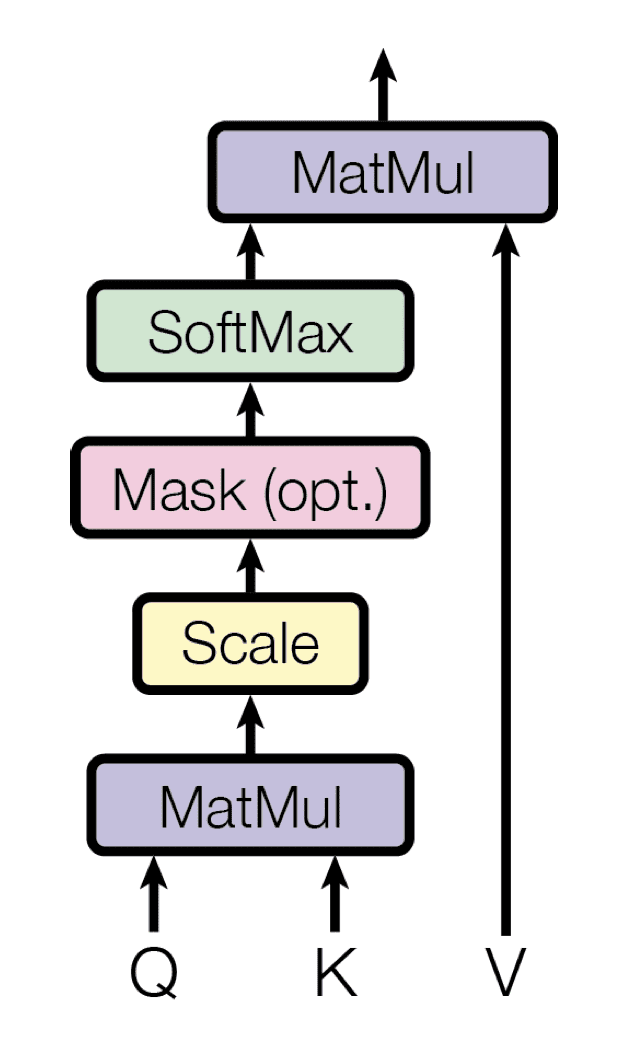
\includegraphics[scale=0.2]{../sections/transformer-architecture/attachments/scaled-dot-product-attention.png}\caption{Illustration of the scaled dot-product attention mechanism. Given query $\mathbf{Q}$, key $\mathbf{K}$, and value $\mathbf{V}$ matrices, the attention scores are computed by performing a matrix multiplication between $\mathbf{Q}$ and $\mathbf{K}^T$, followed by a scaling factor $\frac{1}{\sqrt{d_k}}$ to stabilise gradients. An optional masking step is applied in the decoder to prevent positions from attending to future tokens. The scores are then passed through a softmax function to generate attention weights, which are used to weight the value $\mathbf{V}$ matrix. The final attention output is obtained via matrix multiplication between the attention weights and $\mathbf{V}$, allowing the model to focus on the most relevant parts of the input sequence.}\label{fig:scaled-dot-product-attention}\end{figure}

\subsection{Multi-Head Attention}

To enhance the model's ability to capture various aspects of relationships between tokens, the transformer employs multiple attention heads. This approach involves projecting the queries, keys, and values into different subspaces and computing attention in parallel. It is given by \begin{equation}\text{MultiHead}(\mathbf{Q},\mathbf{K},\mathbf{V})=\text{Concat}(\text{\textbf{head}}_1,\dots,\text{\textbf{head}}_h)\mathbf{W}^O,\end{equation}\label{eq:multihead} where each attention head is given by \begin{equation*}\text{\textbf{head}}_i=\text{Attention}(\mathbf{Q}\mathbf{W}_i^\mathbf{Q},\mathbf{K}\mathbf{W}_i^\mathbf{K},\mathbf{V}\mathbf{W}_i^\mathbf{V}).\end{equation*} Here, $\mathbf{W}_i^\mathbf{Q}$, $\mathbf{W}_i^\mathbf{K}$, $\mathbf{W}_i^\mathbf{V}$, and $\mathbf{W}^\mathbf{O}$ are learned linear projection matrices.

\subsection{Positional Encoding}

Since the transformer does not have any recurrence or convolution to capture sequence order, positional encodings are added to the input embeddings. They inject information about the token positions using sine and cosine functions. The two functions used are \begin{align}\text{PE}_{(pos,2i)}&=\sin\left(\frac{pos}{10000^{\frac{2i}{d_{model}}}}\right),\label{eq:sine-positional-encoding}\\\text{PE}_{(pos,2i+1)}&=\cos\left(\frac{pos}{10000^{\frac{2i}{d_{model}}}}\right).\label{eq:cosine-positional-encoding}\end{align} where $pos$ represents the position in the sequence and $i$ denotes the dimension index. These functions generate unique positional vectors that the model adds to the word embeddings.

\begin{figure}[htbp]\centering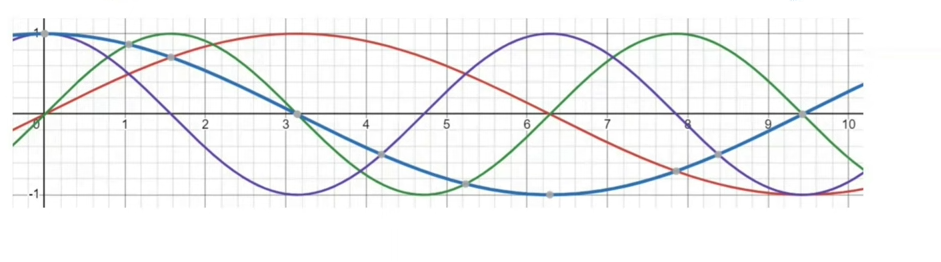
\includegraphics[width=\textwidth]{../sections/transformer-architecture/attachments/positional-encoding.png}\caption{Visualisation of the sine and cosine functions used for positional encoding. Unlike recurrent models, which inherently process sequences step-by-step, transformers lack a built-in notion of order. To overcome this, they use positional encodings, which are added to the input embeddings to provide a unique representation for each position in the sequence. These encodings are generated using sine and cosine functions at different frequencies. The choice of these functions ensure that the encoding captures both absolute and relative positional information. Different frequencies allow the model to recognise repeating patterns and long-range dependencies, even in sequences longer than those seen during training. Since they produce smooth, continuous variations across positions, they provide the model with a structured way to differentiate words based on their position while maintaining meaningful distance relationships between them.}\label{fig:positional-encoding}\end{figure}

\subsection{Feed-Forward Networks}

Each layer in both the encoder and decoder includes a feed-forward network applied to each position independently. This network consists of two linear transformations with a ReLU activation in between. It is given by \begin{equation}\text{FFN}(x)=\max(0,x\mathbf{W}_1+b_1)\mathbf{W}_2+b_2.\end{equation}\label{eq:feed-forward} This component processes the output of the attention mechanisms and adds non-linearity to the model, aiding in the transformation of the attended information.
